% =========================================================================== %
% One Day Tutorial
% =========================================================================== %

\ifx\wholebook\relax\else
  \documentclass[a4paper,10pt,twoside]{book}
  %=============================================================================%
% Common things, settings, packages to include
%=============================================================================%

\usepackage{graphicx}
\usepackage{color}
\usepackage{makeidx}
\usepackage{ifpdf}
\usepackage{verbatim}

% --------------------------------------------------------------------------- %
% Setting up stuff depeding on output format
% --------------------------------------------------------------------------- %

\ifpdf
  % special settings for pdf mode
  \usepackage[colorlinks]{hyperref}
  \usepackage{courier}
  
  \hypersetup{
    colorlinks,
    linkcolor=darkblue,
    citecolor=darkblue,
    pdftitle={The Eclipse Scout Book},
    pdfauthor={The Scout Community},
    pdfkeywords={Enterprise Framework, Eclipse, Java, Client-Side, Rich Client, Web Client, Mobile},
    pdfsubject={Computer Science}
  }
  
  \usepackage{caption}
  \captionsetup{margin=10pt,font=small,labelfont=bf}
\else
  % special stuff for html mode
  \usepackage[tex4ht]{hyperref}
\fi

% --------------------------------------------------------------------------- %
% Setting up printing range
% --------------------------------------------------------------------------- %

\parindent 1cm
\parskip 0.2cm
\topmargin 0.2cm
\oddsidemargin 1cm
\evensidemargin 0.5cm
\textwidth 15cm
\textheight 21cm

% --------------------------------------------------------------------------- %
% Setting up listings
% --------------------------------------------------------------------------- %

\usepackage{listings}
 
\definecolor{darkviolet}{rgb}{0.5,0,0.4}
\definecolor{darkgreen}{rgb}{0,0.4,0.2} 
\definecolor{darkblue}{rgb}{0.1,0.1,0.9}
\definecolor{darkgrey}{rgb}{0.5,0.5,0.5}
\definecolor{lightblue}{rgb}{0.4,0.4,1}
\definecolor{lightgray}{rgb}{0.97,0.97,0.97}

\renewcommand{\lstlistlistingname}{List of Listings}

% general settings
\lstset{
  basicstyle=\small\ttfamily,
  columns=fullflexible,
  breaklines=true,
  breakindent=10pt,
  prebreak=\mbox{{\color{blue}\tiny$\searrow$}},
  postbreak=\mbox{{\color{blue}\tiny$\rightarrow$}},
  showstringspaces=false,
  backgroundcolor=\color{lightgray}
}

% settings for xml files
\lstdefinelanguage{xml}
{
  commentstyle=\color{darkgrey}\upshape,
  morestring=[b]",
  morestring=[s]{>}{<},
  morecomment=[s]{<?}{?>},
  stringstyle=\color{black},
  identifierstyle=\color{darkblue},
  keywordstyle=\color{cyan},
  morekeywords={xmlns,name,point,factory,class}% list your attributes here
}

% settings for ini files
\lstdefinelanguage{ini}
{
  morecomment=[f][\color{darkgrey}\upshape][0]\#, % # is comment iff it's the first char on the line
  stringstyle=\color{black}
}

% default settings (for java files)
\lstset{
  language=Java,
  emphstyle=\color{red}\bfseries,
  keywordstyle=\color{darkviolet}\bfseries,
  commentstyle=\color{darkgreen},
  morecomment=[s][\color{lightblue}]{/**}{*/},
  stringstyle=\color{darkblue},
}

% --------------------------------------------------------------------------- %
% cross reference macros
% --------------------------------------------------------------------------- %
\newcommand{\applabel}[1]{\label{apx:#1}}
\newcommand{\chalabel}[1]{\label{cha:#1}}
\newcommand{\seclabel}[1]{\label{sec:#1}}
\newcommand{\lstlabel}[1]{\label{lst:#1}}
\newcommand{\figlabel}[1]{\label{fig:#1}}
\newcommand{\tablabel}[1]{\label{tab:#1}}

\newcommand{\appref}[1]{Appendix~\ref{apx:#1}}
\newcommand{\charef}[1]{Chapter~\ref{cha:#1}\xspace}
\newcommand{\secref}[1]{Section~\ref{sec:#1}}
\newcommand{\lstref}[1]{Listing~\ref{lst:#1}\xspace}
\newcommand{\figref}[1]{Figure~\ref{fig:#1}\xspace}
\newcommand{\tabref}[1]{Table~\ref{tab:#1}\xspace}

% --------------------------------------------------------------------------- %
% graphics paths
% --------------------------------------------------------------------------- %
\graphicspath{
  {figures/}
  {Introduction/figures/}
}

%=============================================================================%

  \pagestyle{headings}
  \graphicspath{{figures/} {../figures/}}
  \begin{document}
  \sloppy
\fi

% --------------------------------------------------------------------------- %
\chapter{A Larger Example}
\chalabel{large_example}

In this chapter we will create the ''My Contacts'' Scout application.
This small\footnote{
Small in comparison with real world application. But significantly larger and complexer than the ''Hello World'' application of \charef{helloworld}.
} application covers additional aspects of the Eclipse Scout framework. 
The presented demo application borrows heavily from a Scout tutorial published in 2012 the German \textit{Java Magazin}\footnote{
Java Magazin 7.12: \url{https://jaxenter.de/magazines/JavaMagazin72012}.
} 
for the Scout release 3.8 (Juno).
Compared to the 2012 tutorial, the version presented in this chapter has been slightly polished and updated to the Scout release 3.9 (Kepler).

Specifically, we will build an outline based Scout application featuring a navigation tree and pages to present information in tabular form. 
In addition, the application also shows how to work with forms to enter and/or update data, menus and context menus. 
On the server side, we show how to work with databases, how to use logging in Scout applications and how to include standard Java libraries available in JAR files. 

The chapter is organized as follows.
In the first section, the finished demo application is explained from the user perspective. 
The remaining sections focus on the individual steps to implement the ''My Contacts'' application. 
To follow the description of the implementation the reader is assumed to be familiar with the ''Hello World'' tutorial and the Scout SDK as described in \charef{tooling}. 

% --------------------------------------------------------------------------- %
\section{The ''My Contacts'' Application}

The ''My Contacts'' application is a client server application to manage personal contacts. 
Persistece of entered data is achieved through a database backend. 

As social networking services\footnote{
Social networking services in Wikipedia: \url{http://en.wikipedia.org/wiki/Social_network_service}
} 
such as Facebook, LinkedIn or Xing are widely used, the application also provides an example integration with the LinkedIn\footnote{
\url{http://www.linkedin.com/}
} 
plattform. 
The implemented integration allows to download the personal contacts into the local database. 
In the local database it is possible to mix persons entered manually with contact data downloaded from LinkedIn. 

\begin{figure}
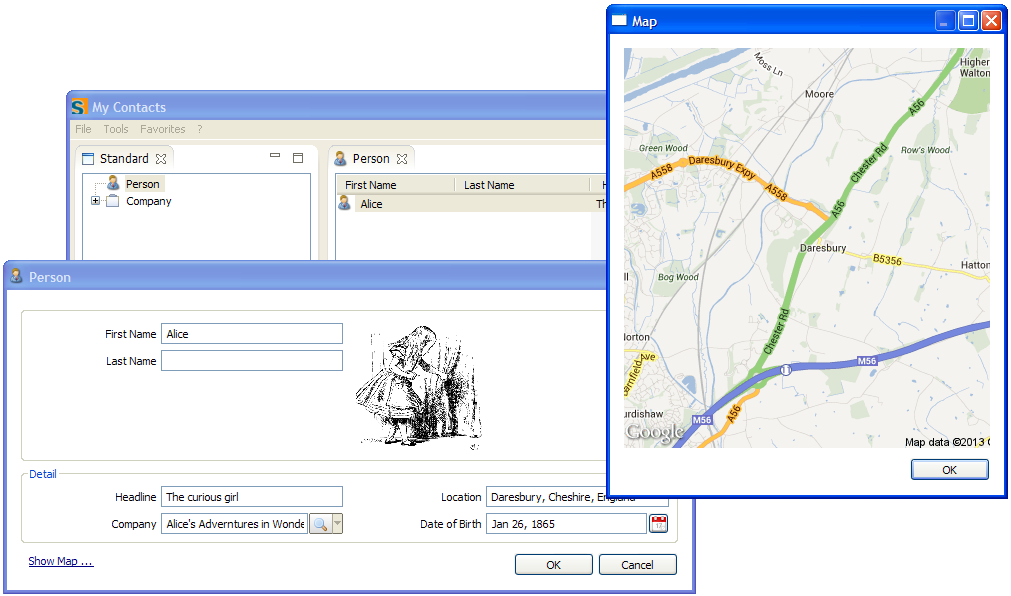
\includegraphics[width=14cm]{my_contacts_swt.png} 
\caption{The SWT client of the ''My Contacts'' application. }
\figlabel{my_contacts_swt}
\end{figure}

After starting the Scout server application a client application may be started that then connects to the server. 
In \figref{my_contacts_swt} the SWT desktop client is shown. 
In the background, the main application window is visible showing a navigation tree on the left hand side. 
On the right side, a table holds the elements corresponding to the selected tree node. 
Using an edit context menu on the selected table row, a form to edit the releant data may be opened as shown in the example screenshot for 'Alice'. 
Clicking on the link 'Show Map ...' in the person form opens the person's location information in a map form using the data provided by Google Maps Image API\footnote{
The Google Maps Image APIs: \url{https://developers.google.com/maps/documentation/imageapis/}.
}.

\begin{figure}
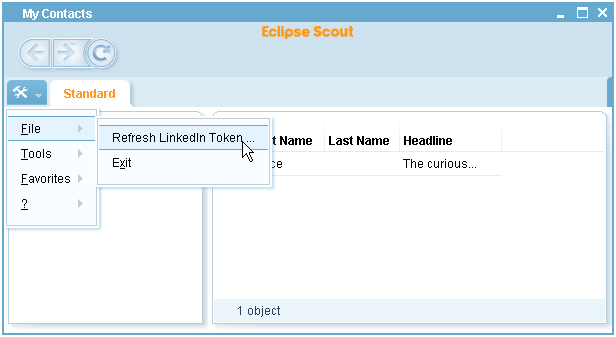
\includegraphics[width=9cm]{my_contacts_rayo_refresh.png} 
\caption{To refresh/generate an access token for reading LinkedIn contacts data select the menu shown in the screenshot. }
\figlabel{my_contacts_rayo_refresh}
\end{figure}

\begin{figure}
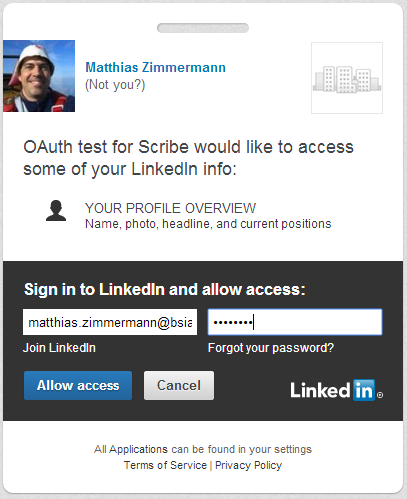
\includegraphics[width=7cm]{my_contacts_rayo_openauthurl.png} \hspace{5mm}
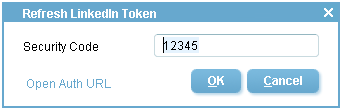
\includegraphics[width=7cm]{my_contacts_rayo_entercode.png}
\caption{To refresh/create the access token click on the provided 'Open Auth URL' link first (left). 
Then, the security code field is enabled and the user can fill in the security code provided on the LinkedIn web page. }
\figlabel{my_contacts_rayo_openauthurl}
\end{figure}

Before any LinkedIn data can be accessed from the ''My Contacts'' application an access token needs to be retrieved from LinkedIn. 
To obtain such a token use the \menu{Refresh LinkedIn Token ...} as shown in \figref{my_contacts_rayo_refresh}. 
This opens the refesh token form shown on the left side of \figref{my_contacts_rayo_openauthurl}. 

\begin{figure}
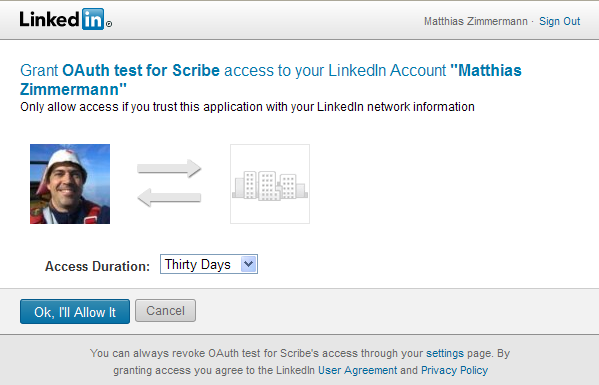
\includegraphics[width=7cm]{oauth_grant_access.png} \hspace{5mm}
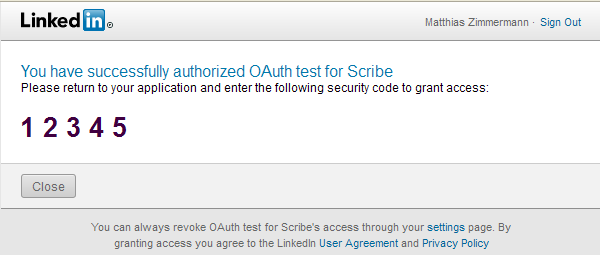
\includegraphics[width=7cm]{oauth_security_code.png} 
\caption{The LinkedIn granting dialog steps shown in a web browser. 
In the first step (right) confirm the access request, then the security code to create an access token is provided in the second step (left).
}
\figlabel{oauth_security_code}
\end{figure}

Clicking on the 'Open Auth URL' link then opens the granting page provided by LinkedIn shown on the left hand side of \figref{oauth_security_code}. 
After logging into your LinkedIn account\footnote{
Yes, for this use case you need a LinkedIn accout. But at least it's free and you will not need to provide very sensitive information such as a mobile phone number, a credit card number or a social security number. 
}
you can specify the desired access duration and confirm the ''OAuth test for Scribe'' access\footnote{
This is the name of the example code provided with the Scribe library that is used with the ''My Contacts'' application. 
} 
to your LinkedIn data.
If the authorization is successful, a security code as shown on the right side of \figref{oauth_security_code} is presented by LinkedIn. 
This code needs then to be entered into the \field{Security Code} as shown on the right side of \figref{my_contacts_rayo_openauthurl}. 
Then, click the \button{OK} to refersh the access token. 

\begin{figure}
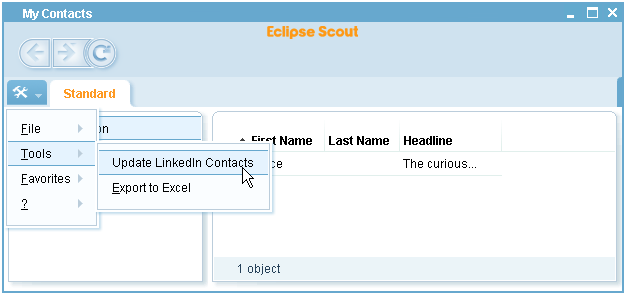
\includegraphics[width=9cm]{my_contacts_rayo_updatecontacts.png} \hspace{5mm}
\caption{Executing the 'Update LinkedIn Contacts for the first time imports the users LinkedIn contacts into the ''My Contacts'' application.}
\figlabel{my_contacts_rayo_updatecontacts}
\end{figure}

To import/update your LinkedIn contacts into your ''My Contacts'' application select the \menu{Update LinkedIn Contacts} as shown in \figref{my_contacts_rayo_updatecontacts}.
Once you have downloaded or entered a number of persons in your ''My Contacts'' application, try to get yourself familiar with the application's person table. 
This is one of the very powerful Scout widgets. 
Columns may be filtered, moved, hidden or sorted (including multi level sort) using the table header context menues \menu{Organize Columns...}  and \menu{Column Filter...}.

Editing and viewing of person data is available by the \contextmenu{Edit Person...} on a selected row.
To manually add a person use the context \contextmenu{New Person...} available on the table header or in the white area outside the displayed columns. 

\begin{figure}
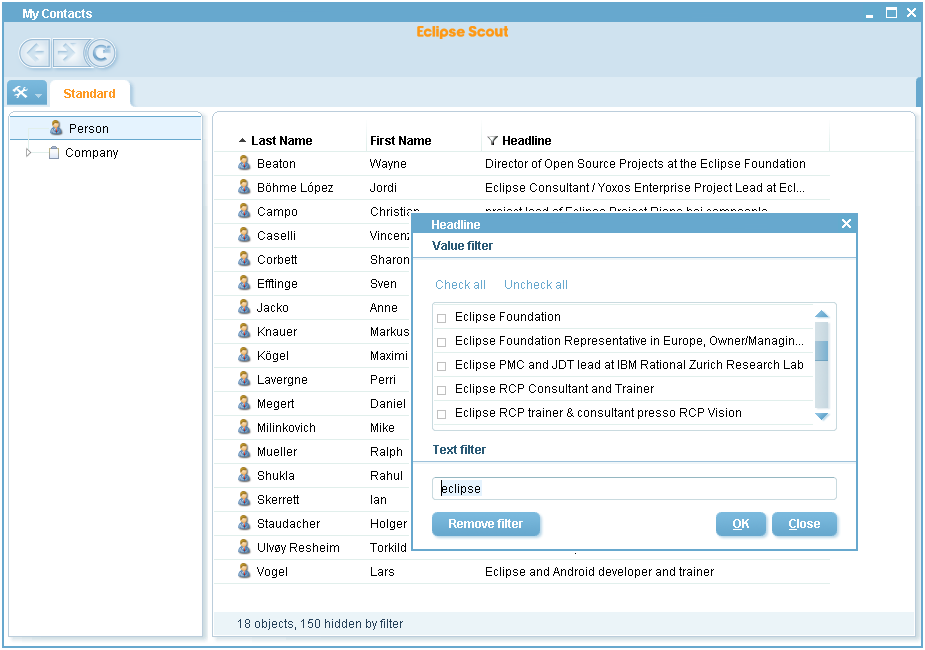
\includegraphics[width=14cm]{my_contacts_rayo_filteredcontacts.png} 
\caption{After importing the contacts from LinkedIn the data is shown in the person page. 
The filter applied on the headline column is indicated by the filter icon. In the front, the filter form shows the filter criterial 'Eclipse'.}
\figlabel{my_contacts_rayo_filteredcontacts}
\end{figure}

\begin{figure}
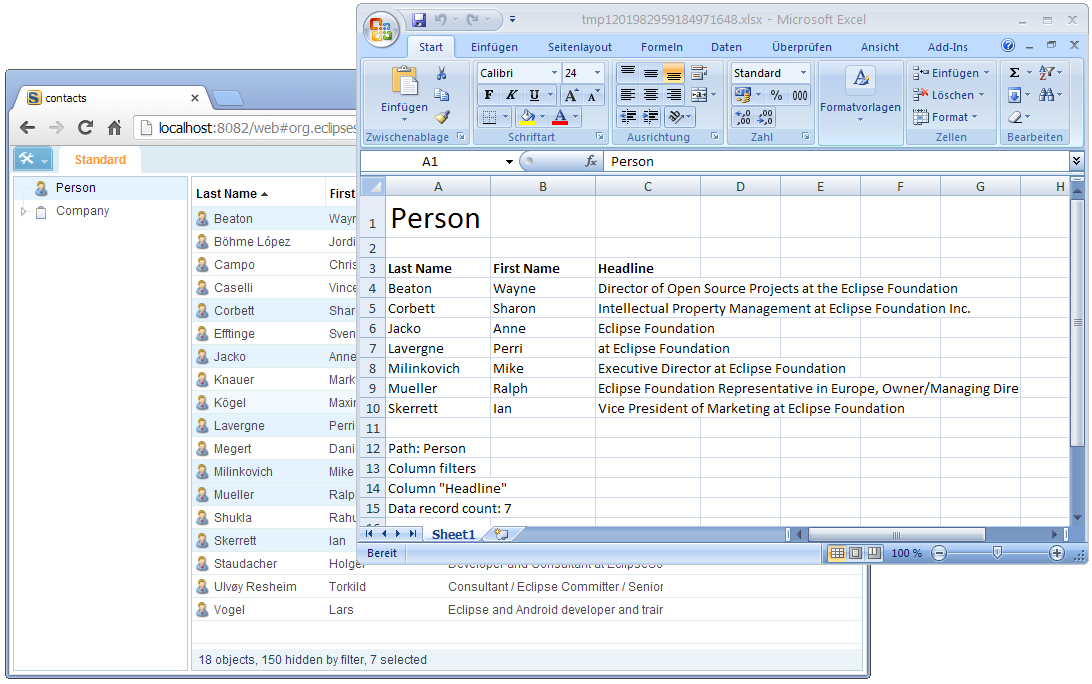
\includegraphics[width=14cm]{my_contacts_rapweb_excelexport.png} 
\caption{The ''My Contacts'' application running in the browser as web application. 
The Excel sheet shown in the front is exported from the person page using the 'Tools/Export to Excel' menu. }
\figlabel{my_contacts_rapweb_excelexport}
\end{figure}

\begin{figure}
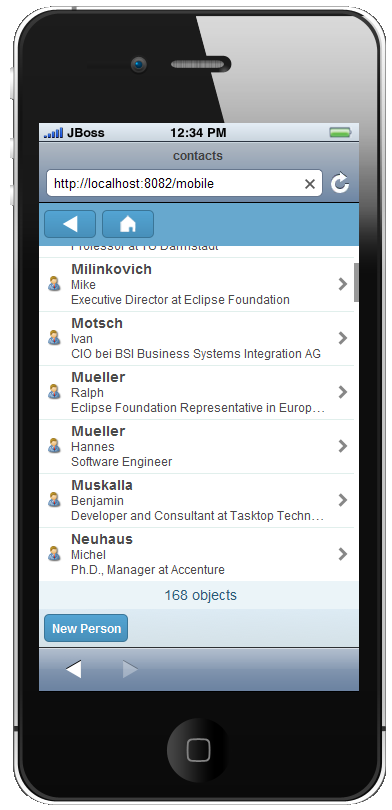
\includegraphics[width=6cm]{my_contacts_rapmobile_1.png} \hspace{5mm}
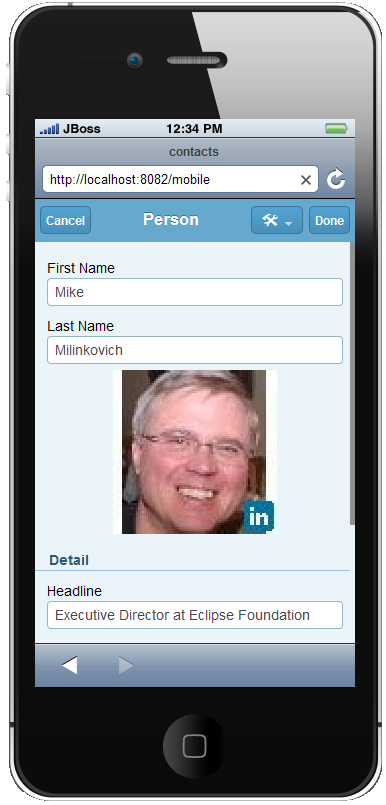
\includegraphics[width=6cm]{my_contacts_rapmobile_2.png} \hspace{5mm}
\caption{The ''My Contacts'' application running on an iPhone device. 
On the left hand side, the person page is shown. The person form is shown on the right. }
\figlabel{my_contacts_rapmobile}
\end{figure}

In \figref{my_contacts_rapweb_excelexport} the ''My Contacts'' application is running in a web browser. 
In this example, the \menu{Tools|Export to to Excel} is used to export the selectd row into an Excel sheet. 
Finally, the ''My Contacts'' application is also running on iPhone and Android mobile devices out of the box. 
Two example screens are provided in \figref{my_contacts_rapmobile}.

Once you no longer feel confident about having the ''My Contacts'' application accessing you data you can revoke this access permission in the LinkedIn menu ''Privacy and Settings''. 
In the lower part of the settings page switch to tab ''Groups, Companies and Applications'' and click on the link ''View your applications''. 
There, you will find again the partner name ''OAuth test for Scribe''. 
To revoke the access, select the associated checkbox and click the ''Remove'' button. 
The next time you try to referesh your LinkedIn data from the ''My Contacts'' application will result in an Error message. 
Before you can again access data from your LinkedIn accout you just need to refresh the access token as described above.

% --------------------------------------------------------------------------- %
\section{Setting up the new Scout project}

\begin{figure}
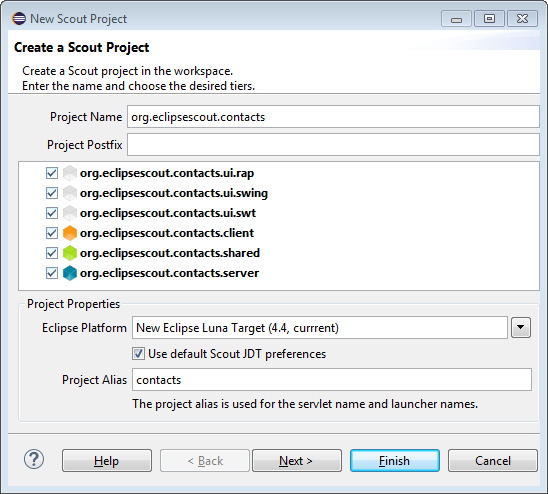
\includegraphics[width=7cm]{new_project_contacts_1.png} \hspace{5mm}
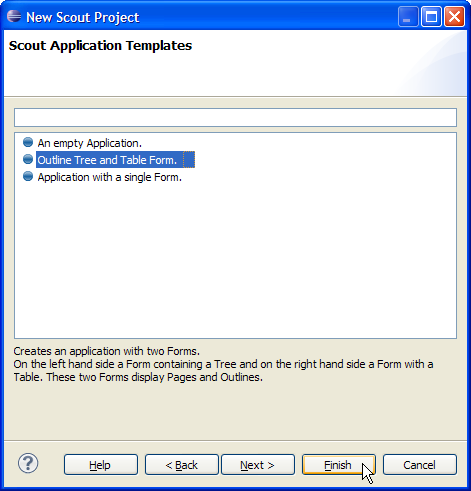
\includegraphics[width=7cm]{new_project_contacts_2.png}
\caption{Start with creating a new Scout project. }
\figlabel{new_project_contacts}
\end{figure}

The initial code for the ''My Contacts'' application is generated using the \wizard{New Scout Project} as decribed in \secref{wizard_new_project}. 
For the \field{Project Name} use the name \java{org.eclipsescout.contacts} as shown on the left side of \figref{new_project_contacts} and click on the \button{Next}. 
In the second wizard step select the application template \element{Outline Tree and Table Form} as shown on the right side of \figref{new_project_contacts}.

\begin{figure}
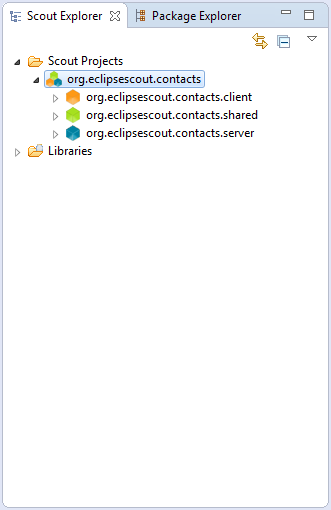
\includegraphics[width=7cm]{project_contacts_explorer.png} \hspace{5mm}
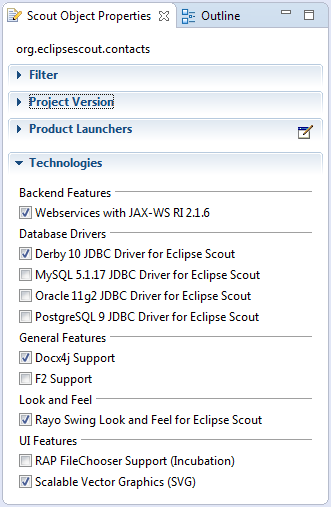
\includegraphics[width=7cm]{project_contacts_properties.png}
\caption{The setting of the \element{Technology} section in the Scout Object Properties of the ''My Contacts'' application.}
\figlabel{project_contacts_properties}
\end{figure}

After the Scout SDK has created the initial application code select the top-level \node{org.eclipsescout.contacts} in the Scout Explorer. 
In the technology section of the corresponding Scout Object Properties select the Derby database driver, the Docx4j support and the Rayo look and feel as shown on the right side of \figref{project_contacts_properties}.
In case you have not yet selected either the Scout Docx4j support or the Rayo look and feel components, the Scout SDK will download these packages from the Eclipse Marketplace\footnote{
See \secref{scout_sdk_object_properties} for additional information regarding the download of marketplace packages}. 

\begin{figure}
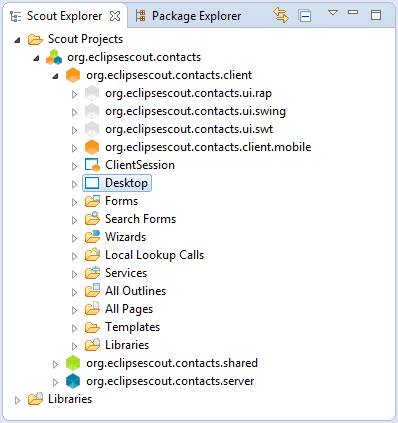
\includegraphics[width=7cm]{desktop_explorer.png} \hspace{5mm}
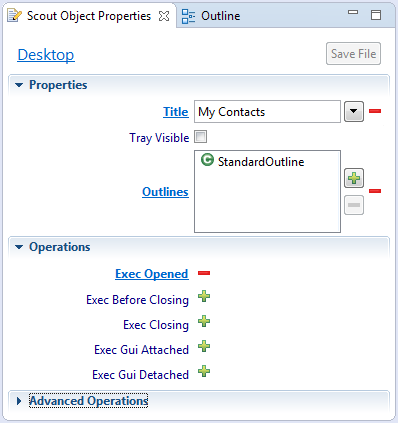
\includegraphics[width=7cm]{desktop_properties.png}
\caption{Configure the application name in the \field{Title} of the Desktop's properties. }
\figlabel{desktop_properties}
\end{figure}

To set the applications name select the \node{Desktop} in the Scout Explorer to access it's Scout Object Properties as shown in \figref{desktop_properties}.
In the \field{Title} enter the string ''My Contacts'' create a new translated text entry. 
Then click on the \link{Exec Opened} in the Scout Object Properties to access the Java code of this method. 

\lstinputlisting[
  label=\lstlabel{mycontacts.desktop.execopened},
  caption=The \java{execOpened} method of desktop class of the "My Contacts" application. The application's organisation into a tree and a table form is defined here.,
  index={execOpened,Desktop,UserAgentUtility},
  linerange={49-70},
  float
]
{../code/oneDayTutorial/org.eclipsescout.contacts.client/src/org/eclipsescout/contacts/client/ui/desktop/Desktop.java}

As shown in \lstref{mycontacts.desktop.execopened} the application's organisation into a tree and a table form is explicitly defined in method \java{execOpened}. 
First, using the \java{UserAgentUtility} class, the method checks if the client is working with a desktop or a web client. 
If not, the method returns and not tree and table setup is used. 
Instead, the \java{MobileHomeForm} defined in plugin \element{org.eclipsescout.contacts.client.mobile} is used. 
In case the user is working with a web client or a desktop client, default tree and table forms are created and started. 
Finally, the currently active outline is set to the \java{StandardOutline}, as this is the only outline defined in this application.

% --------------------------------------------------------------------------- %
\section{Adding the Person Page}

\begin{figure}
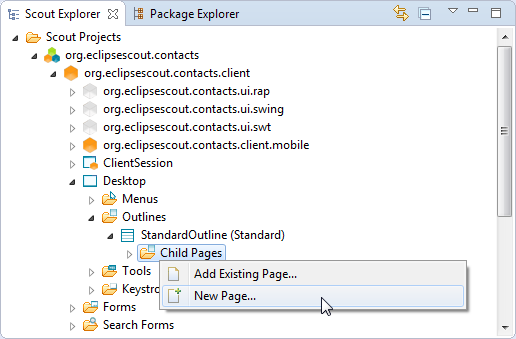
\includegraphics[width=5cm]{new_page_person_contextmenu.png} \hspace{2mm}
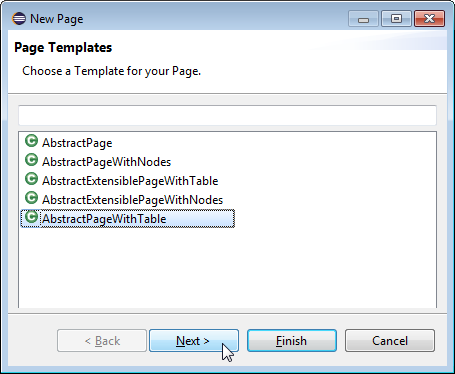
\includegraphics[width=4.5cm]{new_page_person_1.png} \hspace{2mm}
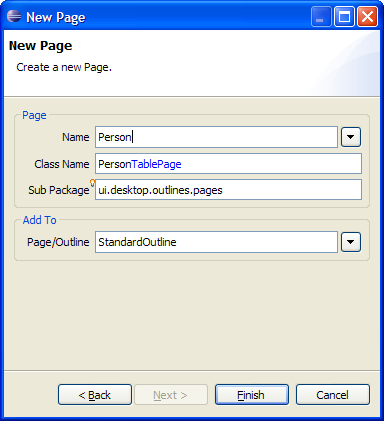
\includegraphics[width=4.5cm]{new_page_person_2.png}
\caption{Add the person table page below the standard outline. }
\figlabel{new_page_person}
\end{figure}

\lstinputlisting[
  label=\lstlabel{mycontacts.desktop.outline.personpage},
  caption=The \java{execCreateChildPages} method of the standard outline. At the current implementation step the company table page is not (yet) added.,
  index={The execCreateChildPages method of the application's standard outline.},
  linerange={19-25},
  float
]
{../code/oneDayTutorial/org.eclipsescout.contacts.client/src/org/eclipsescout/contacts/client/ui/desktop/outlines/StandardOutline.java}

Lorem ipsum will build an outline based Scout application featuring a navigation tree and pages to present information in tabular form. 
In addition, the application also shows how to work with menus and context menus, search forms, and forms to enter and/or update data. 
On the server side we show how to work with databases, how to use logging in Scout applications and how to lorem ipsum. 

\begin{figure}
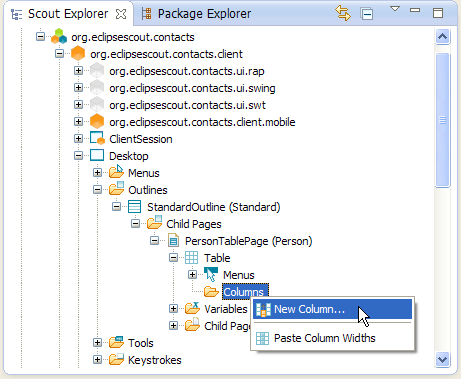
\includegraphics[width=5cm]{new_column_personid_contextmenu.png} \hspace{2mm}
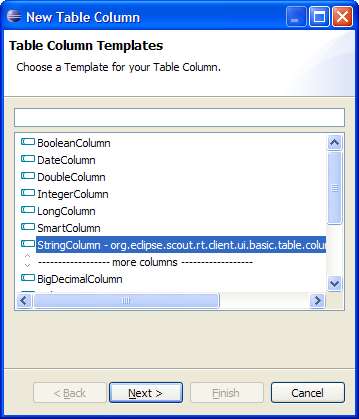
\includegraphics[width=4.5cm]{new_column_personid_1.png} \hspace{2mm}
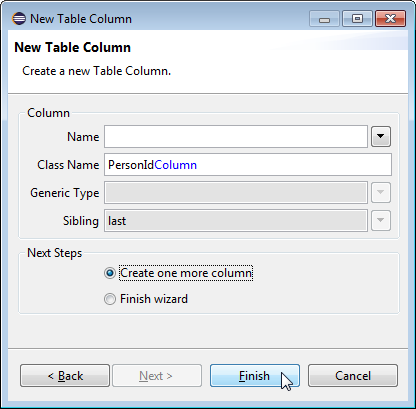
\includegraphics[width=4.5cm]{new_column_personid_2.png}
\caption{Add columns to the person page.}
\figlabel{new_column_personid}
\end{figure}

Lorem ipsum will build an outline based Scout application featuring a navigation tree and pages to present information in tabular form. 
In addition, the application also shows how to work with menus and context menus, search forms, and forms to enter and/or update data. 
On the server side we show how to work with databases, how to use logging in Scout applications and how to lorem ipsum. 

\begin{figure}
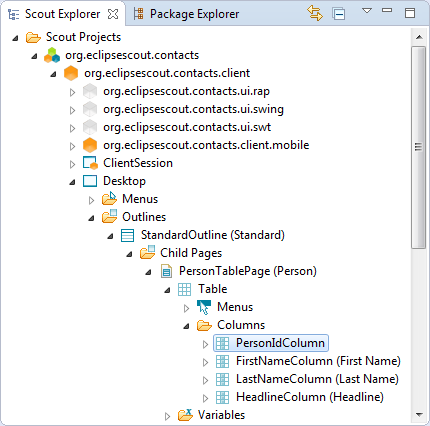
\includegraphics[height=7cm]{person_id_column.png} \hspace{5mm}
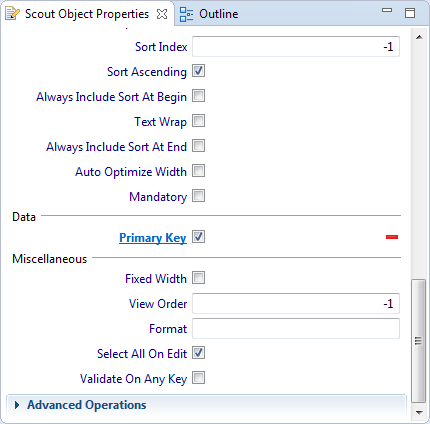
\includegraphics[height=7cm]{person_id_property.png}
\caption{Configure the \element{PersonId} column. Check property \element{Primary Key} under the section \element{Advanced Properties} (right).}
\figlabel{new_column_personid}
\end{figure}

\lstinputlisting[
  label=\lstlabel{mycontacts.desktop.outline.personpage.columns},
  caption=The person id and the first name columns of the \java{PersonTablePage} class. ,
  index={A primary key table column and a default string column.},
  linerange={71-93},
  float
]
{../code/oneDayTutorial/org.eclipsescout.contacts.client/src/org/eclipsescout/contacts/client/ui/desktop/outlines/pages/PersonTablePage.java}

Lorem ipsum will build an outline based Scout application featuring a navigation tree and pages to present information in tabular form. 
In addition, the application also shows how to work with menus and context menus, search forms, and forms to enter and/or update data. 
On the server side we show how to work with databases, how to use logging in Scout applications and how to lorem ipsum. 

\begin{figure}
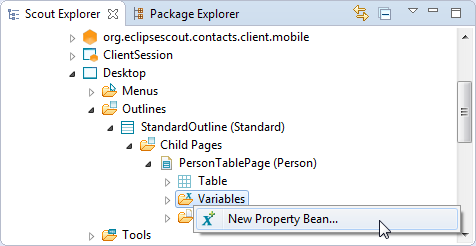
\includegraphics[height=5cm]{new_bean_companyid_contextmenu.png} \hspace{5mm}
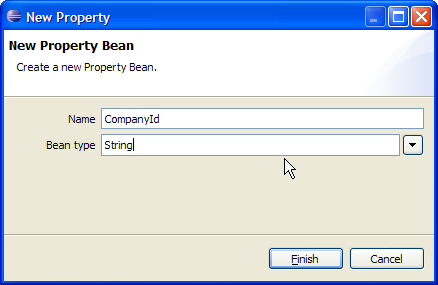
\includegraphics[height=5cm]{new_bean_companyid.png}
\caption{Add the \element{CompanyId} variable to the person page.}
\figlabel{new_bean_companyid}
\end{figure}

\lstinputlisting[
  label=\lstlabel{mycontacts.desktop.outline.personpage.columns},
  caption=The company id variable of the \java{PersonTablePage} class. ,
  index={A table page property bean.},
  linerange={18-20,162-172},
  float
]
{../code/oneDayTutorial/org.eclipsescout.contacts.client/src/org/eclipsescout/contacts/client/ui/desktop/outlines/pages/PersonTablePage.java}

Lorem ipsum will build an outline based Scout application featuring a navigation tree and pages to present information in tabular form. 
In addition, the application also shows how to work with menus and context menus, search forms, and forms to enter and/or update data. 
On the server side we show how to work with databases, how to use logging in Scout applications and how to lorem ipsum. 

% --------------------------------------------------------------------------- %
\section{Adding the Company Page}

\begin{figure}
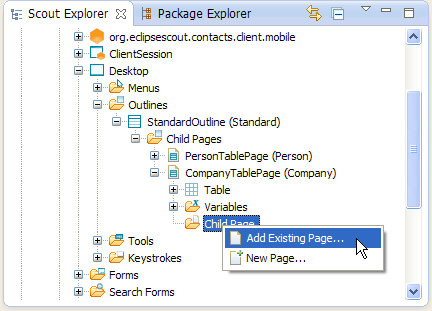
\includegraphics[width=6.5cm]{add_existing_page_contextmenu.png} \hspace{5mm}
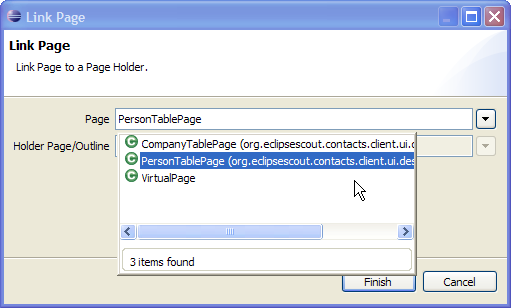
\includegraphics[width=7.5cm]{add_existing_page.png}
\caption{Add the person page below the the company page.}
\figlabel{add_existing_page}
\end{figure}

\lstinputlisting[
  label=\lstlabel{mycontacts.desktop.outline.companypage.linking},
  caption=Linking the \java{PersonTablePage} with the parent \java{CompanyTablePage}.,
  index={Linking pages hierachically.},
  linerange={30-36},
  float
]
{../code/oneDayTutorial/org.eclipsescout.contacts.client/src/org/eclipsescout/contacts/client/ui/desktop/outlines/pages/CompanyTablePage.java}

Lorem ipsum will build an outline based Scout application featuring a navigation tree and pages to present information in tabular form. 
In addition, the application also shows how to work with menus and context menus, search forms, and forms to enter and/or update data. 
On the server side we show how to work with databases, how to use logging in Scout applications and how to lorem ipsum. 


% --------------------------------------------------------------------------- %
\section{Adding the Database in the Server Application}

\begin{figure}
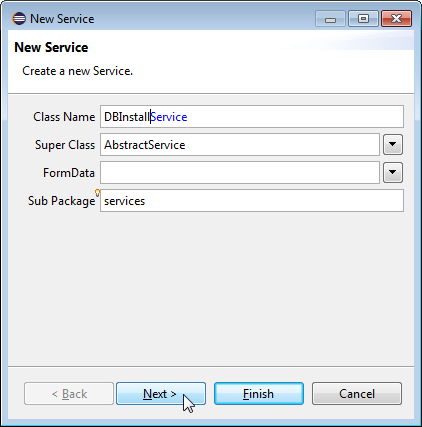
\includegraphics[width=7cm]{new_service_dbinstall_1.png} \hspace{5mm}
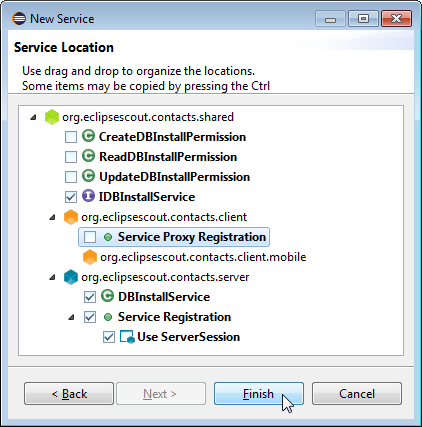
\includegraphics[width=7cm]{new_service_dbinstall_2.png} 
\caption{Add a database installation service. }
\figlabel{new_service_dbinstall}
\end{figure}

Lorem ipsum will build an outline based Scout application featuring a navigation tree and pages to present information in tabular form. 
In addition, the application also shows how to work with menus and context menus, search forms, and forms to enter and/or update data. 
On the server side we show how to work with databases, how to use logging in Scout applications and how to lorem ipsum. 

\begin{figure}
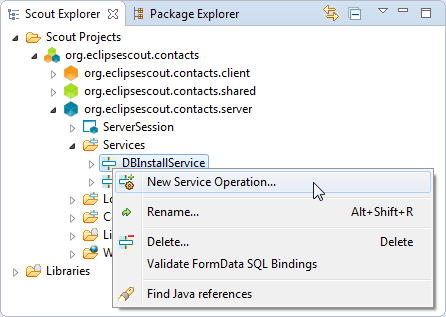
\includegraphics[height=5.5cm]{new_operation_installstorage_contextmenu.png} \hspace{5mm}
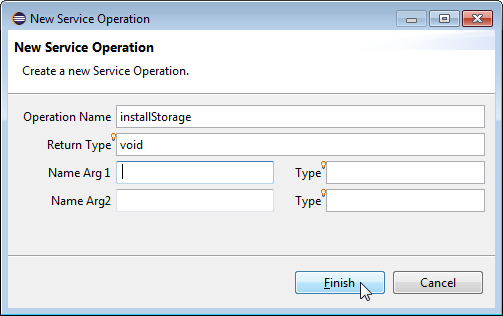
\includegraphics[height=5.5cm]{new_operation_installstorage.png} 
\caption{Add the service operation to create the DB schema. }
\figlabel{new_operation_installstorage}
\end{figure}

\lstinputlisting[
  label=\lstlabel{mycontacts.server.services.installdb},
  caption=The \java{installStorage} service operation to create the database schema for the ''My Contacts'' application.
  New tables are created if they are not found by \java{getExistingTables} in the existing schema.,
  index={A service operation to install a database schema.},
  linerange={14-17,26-36,94-105},
  float
]
{../code/oneDayTutorial/org.eclipsescout.contacts.server/src/org/eclipsescout/contacts/server/services/DBInstallService.java}

Lorem ipsum will build an outline based Scout application featuring a navigation tree and pages to present information in tabular form. 
In addition, the application also shows how to work with menus and context menus, search forms, and forms to enter and/or update data. 
On the server side we show how to work with databases, how to use logging in Scout applications and how to lorem ipsum. 

\lstinputlisting[
  label=\lstlabel{mycontacts.server.services.installdb.company},
  caption=Setting up the \java{COMPANY} table of the ''My Contacts'' application.,
  linerange={37-56},
  float
]
{../code/oneDayTutorial/org.eclipsescout.contacts.server/src/org/eclipsescout/contacts/server/services/DBInstallService.java}

\lstinputlisting[
  label=\lstlabel{mycontacts.server.services.installdb.person},
  caption=Setting up the \java{PERSON} table of the ''My Contacts'' application.,
  linerange={57-79},
  float
]
{../code/oneDayTutorial/org.eclipsescout.contacts.server/src/org/eclipsescout/contacts/server/services/DBInstallService.java}

\lstinputlisting[
  label=\lstlabel{mycontacts.server.services.installdb.users_param},
  caption=Setting up the \java{USERS\_PARAM} table of the ''My Contacts'' application.,
  linerange={80-94},
  float
]
{../code/oneDayTutorial/org.eclipsescout.contacts.server/src/org/eclipsescout/contacts/server/services/DBInstallService.java}

\lstinputlisting[
  label=\lstlabel{mycontacts.server.serverapplication},
  caption=Scheduling the database installation in the \java{start} method of the \java{ServerApplication} class during the server application startup.,
  index={Scheduling a server job during the startup of the Scout server application., ServerApplication},
  linerange={30-57,62-63},
  float
]
{../code/oneDayTutorial/org.eclipsescout.contacts.server/src/org/eclipsescout/contacts/server/ServerApplication.java}

% --------------------------------------------------------------------------- %
\section{Fetching Person and Company Table Data from the Database}

\begin{figure}
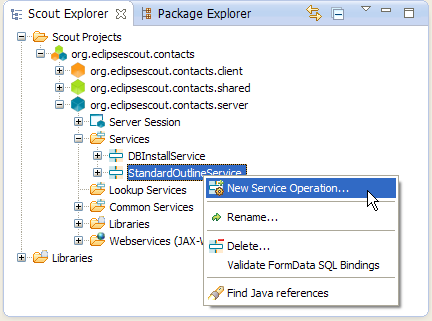
\includegraphics[height=5cm]{new_service_persontabledata_contextmenu.png} \hspace{5mm}
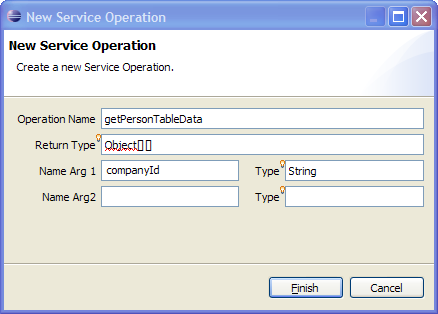
\includegraphics[height=5cm]{new_service_persontabledata.png}
\caption{Add the service operation to fetch the data for the person table. }
\figlabel{new_service_persontabledata}
\end{figure}

Lorem ipsum will build an outline based Scout application featuring a navigation tree and pages to present information in tabular form. 
In addition, the application also shows how to work with menus and context menus, search forms, and forms to enter and/or update data. 
On the server side we show how to work with databases, how to use logging in Scout applications and how to lorem ipsum. 

\lstinputlisting[
  label=\lstlabel{mycontacts.server.services.standardoutline},
  caption=Fetching the table data for the person and the company page of the ''My Contacts'' application.
  The list of persons is restricted to employees of a specific company if a company id parameter is provided.,
  index={Server operations to fetch table data from a database., StandardOutlineService},
  linerange={10-29},
  float
]
{../code/oneDayTutorial/org.eclipsescout.contacts.server/src/org/eclipsescout/contacts/server/services/StandardOutlineService.java}

% --------------------------------------------------------------------------- %
\section{Creating the Person Form}

\begin{figure}
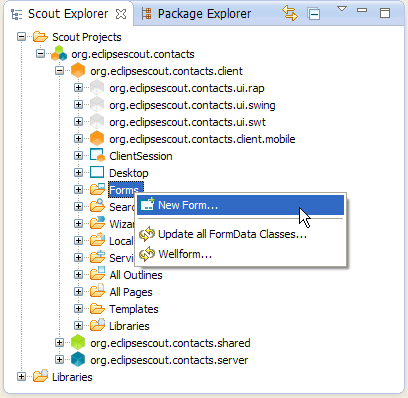
\includegraphics[height=7cm]{new_form_person_contextmenu.png} \hspace{5mm}
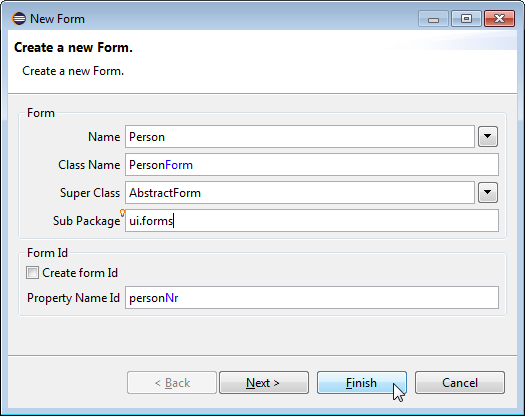
\includegraphics[height=7cm]{new_form_person.png}
\caption{Add the person form.}
\figlabel{new_form_person}
\end{figure}

Lorem ipsum will build an outline based Scout application featuring a navigation tree and pages to present information in tabular form. 
In addition, the application also shows how to work with menus and context menus, search forms, and forms to enter and/or update data. 
On the server side we show how to work with databases, how to use logging in Scout applications and how to lorem ipsum. 

\begin{figure}
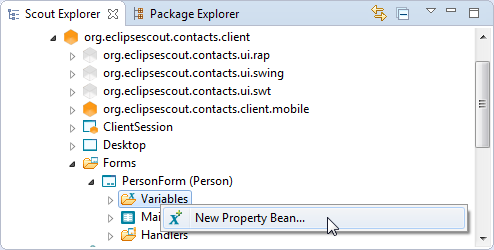
\includegraphics[height=4.5cm]{new_bean_personid_contextmenu.png} \hspace{5mm}
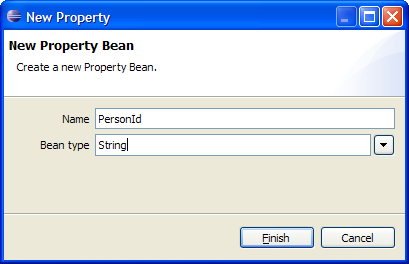
\includegraphics[height=4.5cm]{new_bean_personid.png}
\caption{Add the \element{PersonId} variable to the person form.}
\figlabel{new_bean_personid}
\end{figure}

Lorem ipsum will build an outline based Scout application featuring a navigation tree and pages to present information in tabular form. 
In addition, the application also shows how to work with menus and context menus, search forms, and forms to enter and/or update data. 
On the server side we show how to work with databases, how to use logging in Scout applications and how to lorem ipsum. 

\begin{figure}
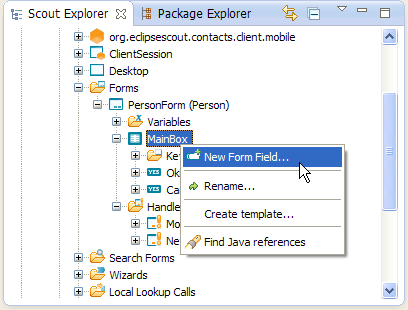
\includegraphics[width=7cm]{new_field_personbox.png} \hspace{5mm}
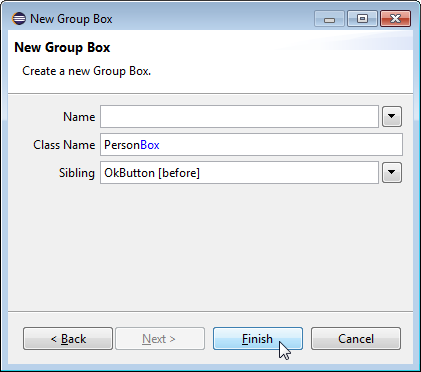
\includegraphics[width=7cm]{new_field_personbox_name.png}
\caption{Add the first group box field to the person form.}
\figlabel{new_field_personbox}
\end{figure}

Lorem ipsum will build an outline based Scout application featuring a navigation tree and pages to present information in tabular form. 
In addition, the application also shows how to work with menus and context menus, search forms, and forms to enter and/or update data. 
On the server side we show how to work with databases, how to use logging in Scout applications and how to lorem ipsum. 

\begin{figure}
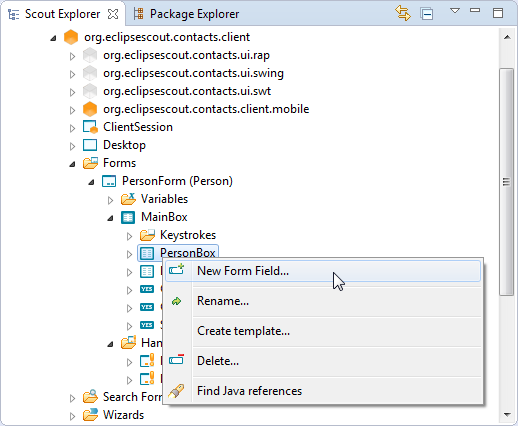
\includegraphics[width=7cm]{new_field_picture_contextmenu.png} \hspace{5mm}
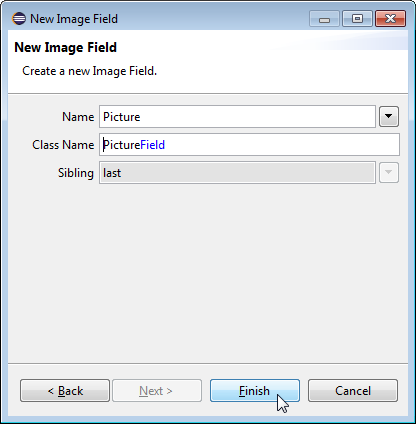
\includegraphics[width=7cm]{new_field_picture.png}
\caption{Add the picture field to the first group box of the person form.}
\figlabel{new_field_picture}
\end{figure}

\lstinputlisting[
  label=\lstlabel{mycontacts.client.forms.person.picturefield},
  caption=The behaviour of the person form's \java{PictureField} is triggered by changes in field \java{PictureUrlField}.,
  index={getConfiguredMasterField, execChangedMasterValue, IOUtility},
  linerange={133-135,151-167,186-187},
  float
]
{../code/oneDayTutorial/org.eclipsescout.contacts.client/src/org/eclipsescout/contacts/client/ui/forms/PersonForm.java}

Lorem ipsum will build an outline based Scout application featuring a navigation tree and pages to present information in tabular form. 
In addition, the application also shows how to work with menus and context menus, search forms, and forms to enter and/or update data. 
On the server side we show how to work with databases, how to use logging in Scout applications and how to lorem ipsum. 

\begin{figure}
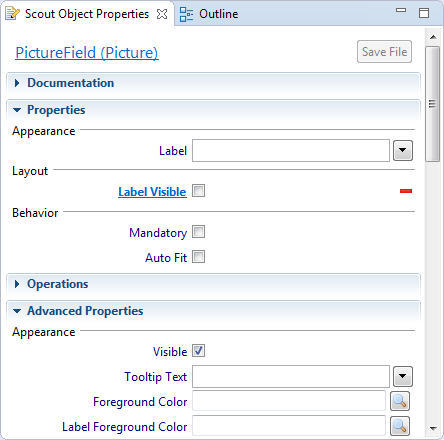
\includegraphics[width=7cm]{picture_field_properties_1.png} \hspace{5mm}
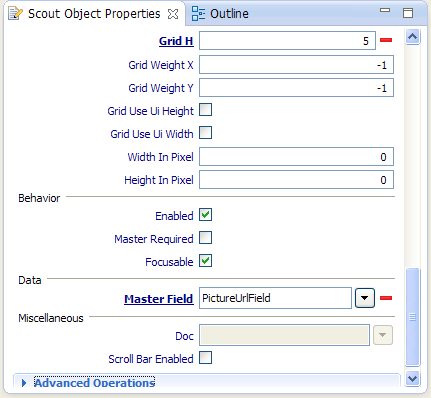
\includegraphics[width=7cm]{picture_field_properties_2.png}
\caption{Set the properties for the picture field of the person form.}
\figlabel{picture_field_properties}
\end{figure}

\lstinputlisting[
  label=\lstlabel{mycontacts.client.forms.person.picturefield.properties},
  caption=The Java code for the selected Scout Object Properties of the \java{PictureField}.,
  index={getConfiguredMasterField, execChangedMasterValue, IOUtility},
  linerange={133-150,186-187},
  float
]
{../code/oneDayTutorial/org.eclipsescout.contacts.client/src/org/eclipsescout/contacts/client/ui/forms/PersonForm.java}

Lorem ipsum will build an outline based Scout application featuring a navigation tree and pages to present information in tabular form. 
In addition, the application also shows how to work with menus and context menus, search forms, and forms to enter and/or update data. 
On the server side we show how to work with databases, how to use logging in Scout applications and how to lorem ipsum. 

\begin{figure}
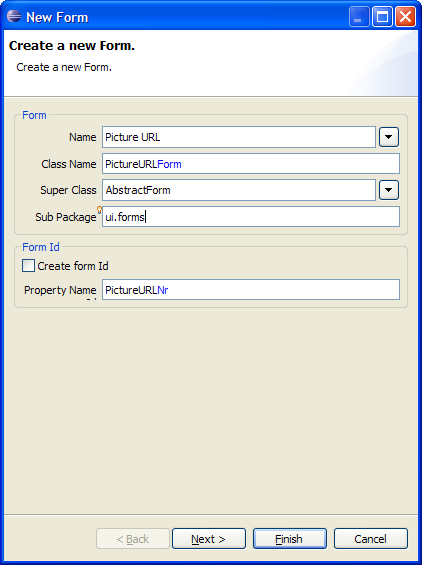
\includegraphics[width=7cm]{new_form_url_1.png} \hspace{5mm}
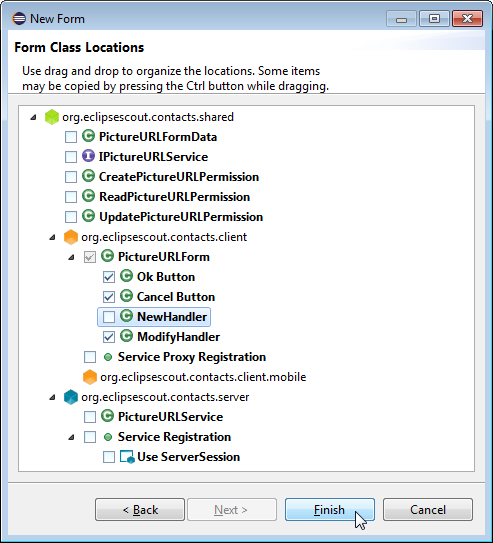
\includegraphics[width=7cm]{new_form_url_2.png}
\caption{Add the URL editor form.}
\figlabel{new_form_url}
\end{figure}

\lstinputlisting[
  label=\lstlabel{mycontacts.client.forms.pictureurl},
  caption=The UI structure of the \java{PictureURLForm} used to update the URL of the picture field in the person form.,
  linerange={17-18,52-67,79-80},
  float
]
{../code/oneDayTutorial/org.eclipsescout.contacts.client/src/org/eclipsescout/contacts/client/ui/forms/PictureURLForm.java}

Lorem ipsum will build an outline based Scout application featuring a navigation tree and pages to present information in tabular form. 
In addition, the application also shows how to work with menus and context menus, search forms, and forms to enter and/or update data. 
On the server side we show how to work with databases, how to use logging in Scout applications and how to lorem ipsum. 

\begin{figure}
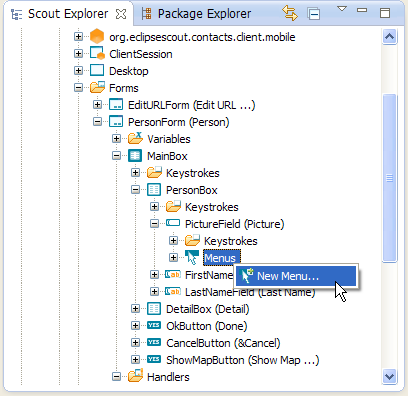
\includegraphics[width=7cm]{new_menu_editurl_contextmenu.png} \hspace{5mm}
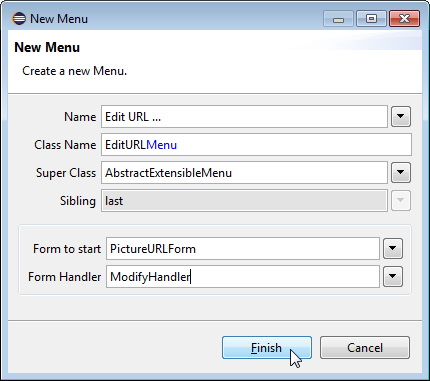
\includegraphics[width=7cm]{new_menu_editurl.png}
\caption{Add the URL edit menu to the picture field.}
\figlabel{new_menu_editurl}
\end{figure}

\lstinputlisting[
  label=\lstlabel{mycontacts.client.forms.person.picturefield.editmenu},
  caption=The edit menu implemented in class \java{EditURLMenu} of the picture field.
  If the URL was changed the picture URL field of the person form is set accordingly in method \java{execAction},
  index={execAction},
  linerange={168-185},
  float
]
{../code/oneDayTutorial/org.eclipsescout.contacts.client/src/org/eclipsescout/contacts/client/ui/forms/PersonForm.java}

Lorem ipsum will build an outline based Scout application featuring a navigation tree and pages to present information in tabular form. 
In addition, the application also shows how to work with menus and context menus, search forms, and forms to enter and/or update data. 
On the server side we show how to work with databases, how to use logging in Scout applications and how to lorem ipsum. 

% --------------------------------------------------------------------------- %
\section{Integrating the Person Form into the Application}

\begin{figure}
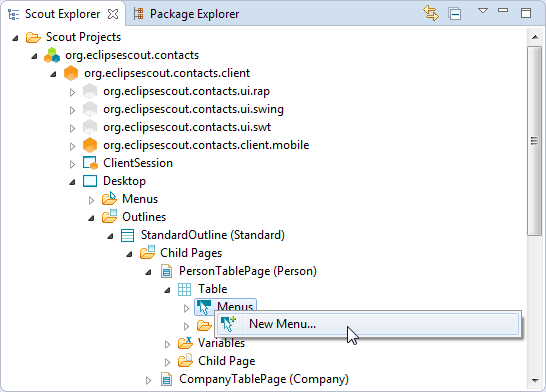
\includegraphics[width=7cm]{new_menu_editperson_contextmenu.png} \hspace{5mm}
\includegraphics[width=7cm]{new_menu_editperson.png}
\caption{Add the Person edit menu to the person page.}
\figlabel{new_menu_editperson}
\end{figure}

\lstinputlisting[
  label=\lstlabel{mycontacts.desktop.outline.personpage.editmenu},
  caption=The \java{EditPersonMenu} to edit the person selected in the person table.
  The person id taken from the corresponding (invisible) column is transferred to the person form before the form is started.,
  index={isFormStored, reloadPage},
  linerange={112-131},
  float
]
{../code/oneDayTutorial/org.eclipsescout.contacts.client/src/org/eclipsescout/contacts/client/ui/desktop/outlines/pages/PersonTablePage.java}

Lorem ipsum will build an outline based Scout application featuring a navigation tree and pages to present information in tabular form. 
In addition, the application also shows how to work with menus and context menus, search forms, and forms to enter and/or update data. 
On the server side we show how to work with databases, how to use logging in Scout applications and how to lorem ipsum. 

\begin{figure}
\includegraphics[height=5cm]{person_table_explorer.png} \hspace{5mm}
\includegraphics[height=5cm]{person_table_properties.png}
\caption{Set the behaviour for the row level action on the person table.}
\figlabel{person_table_properties}
\end{figure}

\lstinputlisting[
  label=\lstlabel{mycontacts.desktop.outline.personpage.execrowaction},
  caption=The \java{execRowAction} method on table pages is used to trigger an action when a row is selcted with a double click or \textsc{<Enter>}.,
  index={execRowAction},
  linerange={58-62},
  float
]
{../code/oneDayTutorial/org.eclipsescout.contacts.client/src/org/eclipsescout/contacts/client/ui/desktop/outlines/pages/PersonTablePage.java}

Lorem ipsum will build an outline based Scout application featuring a navigation tree and pages to present information in tabular form. 
In addition, the application also shows how to work with menus and context menus, search forms, and forms to enter and/or update data. 
On the server side we show how to work with databases, how to use logging in Scout applications and how to lorem ipsum. 

% --------------------------------------------------------------------------- %
\section{Extending the Person Form with a Company Smartfield}

\begin{figure}
\includegraphics[width=6cm]{new_lookupcall_company_contextmenu.png}
\caption{Add a lookup call to the applications shared node.}
\figlabel{new_lookupcall_company_contextmenu}
\end{figure}

\begin{figure}
\includegraphics[height=5.5cm]{new_lookupcall_company_1.png} \hspace{5mm}
\includegraphics[height=5.5cm]{new_lookupcall_company_2.png}
\caption{The two wizard steps to enter the details of the company lookup call.}
\figlabel{new_lookupcall_company}
\end{figure}

\lstinputlisting[
  label=\lstlabel{mycontacts.shared.lookup.companylookupcall},
  caption=The company lookup call with its \java{getConfiguredService} method in the application's shared plugin.,
  index={LookupCall, getConfiguredService},
  linerange={7-16},
  float
]
{../code/oneDayTutorial/org.eclipsescout.contacts.shared/src/org/eclipsescout/contacts/shared/services/lookup/CompanyLookupCall.java}

\lstinputlisting[
  label=\lstlabel{mycontacts.server.lookup.companylookupservice},
  caption=The company lookup service in the application's server plugin.
  The \java{key} and the \java{text} criterias are used to search for values by key or by the provided name substring.
  index={AbstractSqlLookupService, getConfiguredSqlSelect},
  linerange={6-20},
  float
]
{../code/oneDayTutorial/org.eclipsescout.contacts.server/src/org/eclipsescout/contacts/server/services/lookup/CompanyLookupService.java}

Lorem ipsum will build an outline based Scout application featuring a navigation tree and pages to present information in tabular form. 
In addition, the application also shows how to work with menus and context menus, search forms, and forms to enter and/or update data. 
On the server side we show how to work with databases, how to use logging in Scout applications and how to lorem ipsum. 

\begin{figure}
\includegraphics[width=7cm]{new_smartfield_company_contextmenu.png}
\caption{Add a smartfield to the person form.}
\figlabel{new_smartfield_company_contextmenu}
\end{figure}

\begin{figure}
\includegraphics[height=5cm]{new_smartfield_company_1.png} \hspace{5mm}
\includegraphics[height=5cm]{new_smartfield_company_2.png}
\caption{Create the company smartfield for the person form.}
\figlabel{new_smartfield_company}
\end{figure}

\lstinputlisting[
  label=\lstlabel{mycontacts.client.forms.person.companyfield},
  caption=The smartfield \java{CompanyField} of the person form and its wiring with the company lookup call.,
  index={AbstractSmartField, getConfiguredLookupCall},
  linerange={233-247},
  float
]
{../code/oneDayTutorial/org.eclipsescout.contacts.client/src/org/eclipsescout/contacts/client/ui/forms/PersonForm.java}

Lorem ipsum will build an outline based Scout application featuring a navigation tree and pages to present information in tabular form. 
In addition, the application also shows how to work with menus and context menus, search forms, and forms to enter and/or update data. 
On the server side we show how to work with databases, how to use logging in Scout applications and how to lorem ipsum. 


% --------------------------------------------------------------------------- %
\section{Adding the Scribe Library to the Application}

\begin{figure}
\includegraphics[width=7cm]{new_library_scribe_contextmenu.png} \hspace{5mm}
\caption{Add a new bundle to hold the Scribe JARs.}
\figlabel{new_library_scribe_contextmenu}
\end{figure}

Lorem ipsum will build an outline based Scout application featuring a navigation tree and pages to present information in tabular form. 
In addition, the application also shows how to work with menus and context menus, search forms, and forms to enter and/or update data. 
On the server side we show how to work with databases, how to use logging in Scout applications and how to lorem ipsum. 

\begin{figure}
\includegraphics[width=7cm]{new_library_scribe_1.png} \hspace{5mm}
\includegraphics[width=7cm]{new_library_scribe_2.png}
\caption{Specify the JARs to be contained in the library bundle and the library name.}
\figlabel{new_library_scribe}
\end{figure}

Lorem ipsum will build an outline based Scout application featuring a navigation tree and pages to present information in tabular form. 
In addition, the application also shows how to work with menus and context menus, search forms, and forms to enter and/or update data. 
On the server side we show how to work with databases, how to use logging in Scout applications and how to lorem ipsum. 

% --------------------------------------------------------------------------- %
\section{Integrating LinkedIn Access with Scribe}

\begin{figure}
\includegraphics[height=5.5cm]{new_operation_authurl_contextmenu.png} \hspace{5mm}
\includegraphics[height=5.5cm]{new_operation_authurl.png}
\caption{Add the operation to retrieve an authentication URL.}
\figlabel{new_operation_authurl}
\end{figure}

\lstinputlisting[
  label=\lstlabel{mycontacts.server.linkedin.initialize},
  caption=The \java{LinkedInService} service with it's \java{initializeService} method defined in the \java{IService} interface.,
  index={IService, initializeService},
  linerange={32-50,160-161},
  float
]
{../code/oneDayTutorial/org.eclipsescout.contacts.server/src/org/eclipsescout/contacts/server/services/LinkedInService.java}

\lstinputlisting[
  label=\lstlabel{mycontacts.server.linkedin.authurl},
  caption=The \java{getAuthUrl} method of the LinkedIn service.,
  index={AbstractSmartField, getConfiguredLookupCall},
  linerange={51-57},
  float
]
{../code/oneDayTutorial/org.eclipsescout.contacts.server/src/org/eclipsescout/contacts/server/services/LinkedInService.java}

Lorem ipsum will build an outline based Scout application featuring a navigation tree and pages to present information in tabular form. 
In addition, the application also shows how to work with menus and context menus, search forms, and forms to enter and/or update data. 
On the server side we show how to work with databases, how to use logging in Scout applications and how to lorem ipsum. 

\begin{figure}
\includegraphics[height=5.5cm]{new_operation_refreshtoken.png} \hspace{5mm}
\includegraphics[height=5.5cm]{new_operation_updatecontacts.png}
\caption{Add the operations to refresh the access token and to update the LinkedIn contacts.}
\figlabel{new_operation_refresh_update}
\end{figure}

\lstinputlisting[
  label=\lstlabel{mycontacts.server.linkedin.refreshtoken},
  caption=The \java{refreshToken} method is used to create a new access token to fetch data from the LinkedIn API.,
  linerange={58-85},
  float
]
{../code/oneDayTutorial/org.eclipsescout.contacts.server/src/org/eclipsescout/contacts/server/services/LinkedInService.java}

\lstinputlisting[
  label=\lstlabel{mycontacts.server.linkedin.updatecontacts},
  caption=The \java{updateContacts} method is used to enter/update existing contacts based on new data fetched from LinkedIn.,
  linerange={86-122},
  float
]
{../code/oneDayTutorial/org.eclipsescout.contacts.server/src/org/eclipsescout/contacts/server/services/LinkedInService.java}

\lstinputlisting[
  label=\lstlabel{mycontacts.server.linkedin.readcontacts},
  caption=The \java{readContacts} method to fetch the users connection using the LinkedIn API.
  The necessary access token is created in method \java{getToken} based on the information stored in the database for the logged in user.,
  linerange={123-159},
  float
]
{../code/oneDayTutorial/org.eclipsescout.contacts.server/src/org/eclipsescout/contacts/server/services/LinkedInService.java}

\lstinputlisting[
  label=\lstlabel{mycontacts.server.linkedin.domutil},
  caption=The \java{DomUtility} class provides functions to parse the XML data structure provided by the LinkedIn API.,
  linerange={13-45},
  float
]
{../code/oneDayTutorial/org.eclipsescout.contacts.server/src/org/eclipsescout/contacts/server/services/DomUtility.java}

\begin{lstlisting}[backgroundcolor=\color{white},language=xml]
<?xml version="1.0" encoding="UTF-16"?>
<person>
    <id>f7R6wGcblj</id>
    <first-name>Mike</first-name>
    <last-name>Milinkovich</last-name>
    <headline>Executive Director at Eclipse Foundation</headline>
    <picture-url>http://m3.licdn.com/mpr/mprx/0_IUM7Se9vBU...SbRbQZ4</picture-url>
    <site-standard-profile-request>
      <url>http://www.linkedin.com/profile/view?id=14949387...05720*s114280*</url>
    </site-standard-profile-request>
    <location>
      <name>Ottawa, Canada Area</name>
      <country>
        <code>ca</code>
      </country>
    </location>
    <industry>Computer Software</industry>
  </person>
\end{lstlisting}

Lorem ipsum will build an outline based Scout application featuring a navigation tree and pages to present information in tabular form. 
In addition, the application also shows how to work with menus and context menus, search forms, and forms to enter and/or update data. 
On the server side we show how to work with databases, how to use logging in Scout applications and how to lorem ipsum. 

\begin{figure}
\includegraphics[width=7cm]{new_form_token_1.png} \hspace{5mm}
\includegraphics[width=7cm]{new_form_token_2.png}
\caption{Add the form to refresh the LinkedIn access token.}
\figlabel{new_form_token}
\end{figure}

Lorem ipsum will build an outline based Scout application featuring a navigation tree and pages to present information in tabular form. 
In addition, the application also shows how to work with menus and context menus, search forms, and forms to enter and/or update data. 
On the server side we show how to work with databases, how to use logging in Scout applications and how to lorem ipsum. 

\begin{figure}
\includegraphics[width=7cm]{tokenform_securitycode_explorer.png} \hspace{5mm}
\includegraphics[width=7cm]{tokenform_securitycode_properties.png}
\caption{The token form in the explorer and the properties of the security code field.}
\figlabel{tokenform_securitycode}
\end{figure}

\lstinputlisting[
  label=\lstlabel{mycontacts.client.forms.refreshtoken},
  caption=The structure of the refersh token form. The security code field gets enabled in method \java{execClickAction} after the authentication link button is pressed.,
  index={AbstractLinkButton,execClickAction},
  linerange={23-25,65-104},
  float
]
{../code/oneDayTutorial/org.eclipsescout.contacts.client/src/org/eclipsescout/contacts/client/ui/forms/RefreshTokenForm.java}

Lorem ipsum will build an outline based Scout application featuring a navigation tree and pages to present information in tabular form. 
In addition, the application also shows how to work with menus and context menus, search forms, and forms to enter and/or update data. 
On the server side we show how to work with databases, how to use logging in Scout applications and how to lorem ipsum. 

\begin{figure}
\includegraphics[width=7cm]{new_menu_refreshtoken_contextmenu.png} \hspace{5mm}
\includegraphics[width=7cm]{new_menu_refreshtoken.png}
\caption{Add the menu to open the LinkedIn token form.}
\figlabel{new_menu_refreshtoken}
\end{figure}

\lstinputlisting[
  label=\lstlabel{mycontacts.client.desktop.refreshtokenmenu},
  caption=The menu to refresh the LinkedIn token starts the token form and then sends token parameters with the new security code to the LinkedIn backend service.,
  linerange={79-105},
  float
]
{../code/oneDayTutorial/org.eclipsescout.contacts.client/src/org/eclipsescout/contacts/client/ui/desktop/Desktop.java}

Lorem ipsum will build an outline based Scout application featuring a navigation tree and pages to present information in tabular form. 
In addition, the application also shows how to work with menus and context menus, search forms, and forms to enter and/or update data. 
On the server side we show how to work with databases, how to use logging in Scout applications and how to lorem ipsum. 

% --------------------------------------------------------------------------- %
\section{Fetching Contacts from LinkedIn}

\begin{figure}
\includegraphics[width=7cm]{new_menu_updatecontacts_contextmenu.png} \hspace{5mm}
\includegraphics[width=7cm]{new_menu_updatecontacts.png}
\caption{Add the menu to update the LinkedIn contacts.}
\figlabel{new_menu_updatecontacts}
\end{figure}

\lstinputlisting[
  label=\lstlabel{mycontacts.client.desktop.refreshtokenmenu},
  caption=The menu to update the stored persons with current LinkedIn data.,
  linerange={129-144},
  float
]
{../code/oneDayTutorial/org.eclipsescout.contacts.client/src/org/eclipsescout/contacts/client/ui/desktop/Desktop.java}

server first, db setup service
server, derby sql service

server application

config.ini

\ifx\wholebook\relax\else
   \begin{thebibliography}{99}
  \addcontentsline{toc}{chapter}{Bibliography}
  
  % add/insert books in alphabetical order of 1st author
  
  \bibitem{batessierra05}
    \textit{Bert Bates, Kathy Sierra},
	\textbf{Head First Java} 2nd edition, 
	O'Reilly Media, 2005.

  \bibitem{bloch08} 
    \textit{Joshua Bloch},
    \textbf{Effective Java} 2nd edition, 
	Addison-Wesley, 2008.
	
  \bibitem{eckel06}
    \textit{Bruce Eckel},
	\textbf{Thinking in Java} 4th edition, 
	Prentice Hall International, 2006.

\end{thebibliography}

   \end{document}
\fi

% =========================================================================== %
